\documentclass[border=0pt,10pt]{standalone}
\usepackage{tikz}
\usetikzlibrary{backgrounds, calc, patterns}
\renewcommand\rmdefault{\sfdefault}

% define simple color names for esa colors and a highlight
\definecolor{esa}{RGB}{10,156,215}
\def\esacolorfactor{20}
\colorlet{esa0}{esa!90!white}
\colorlet{esa1}{black!\esacolorfactor!esa0}
\colorlet{esa2}{black!\esacolorfactor!esa1}
\colorlet{esa3}{black!\esacolorfactor!esa2}
\colorlet{esa4}{black!\esacolorfactor!esa3}
\colorlet{esa5}{black!\esacolorfactor!esa4}
\definecolor{highlight}{RGB}{189,27,27}



\newcount\mycount
\newcount\numcount
\begin{document}
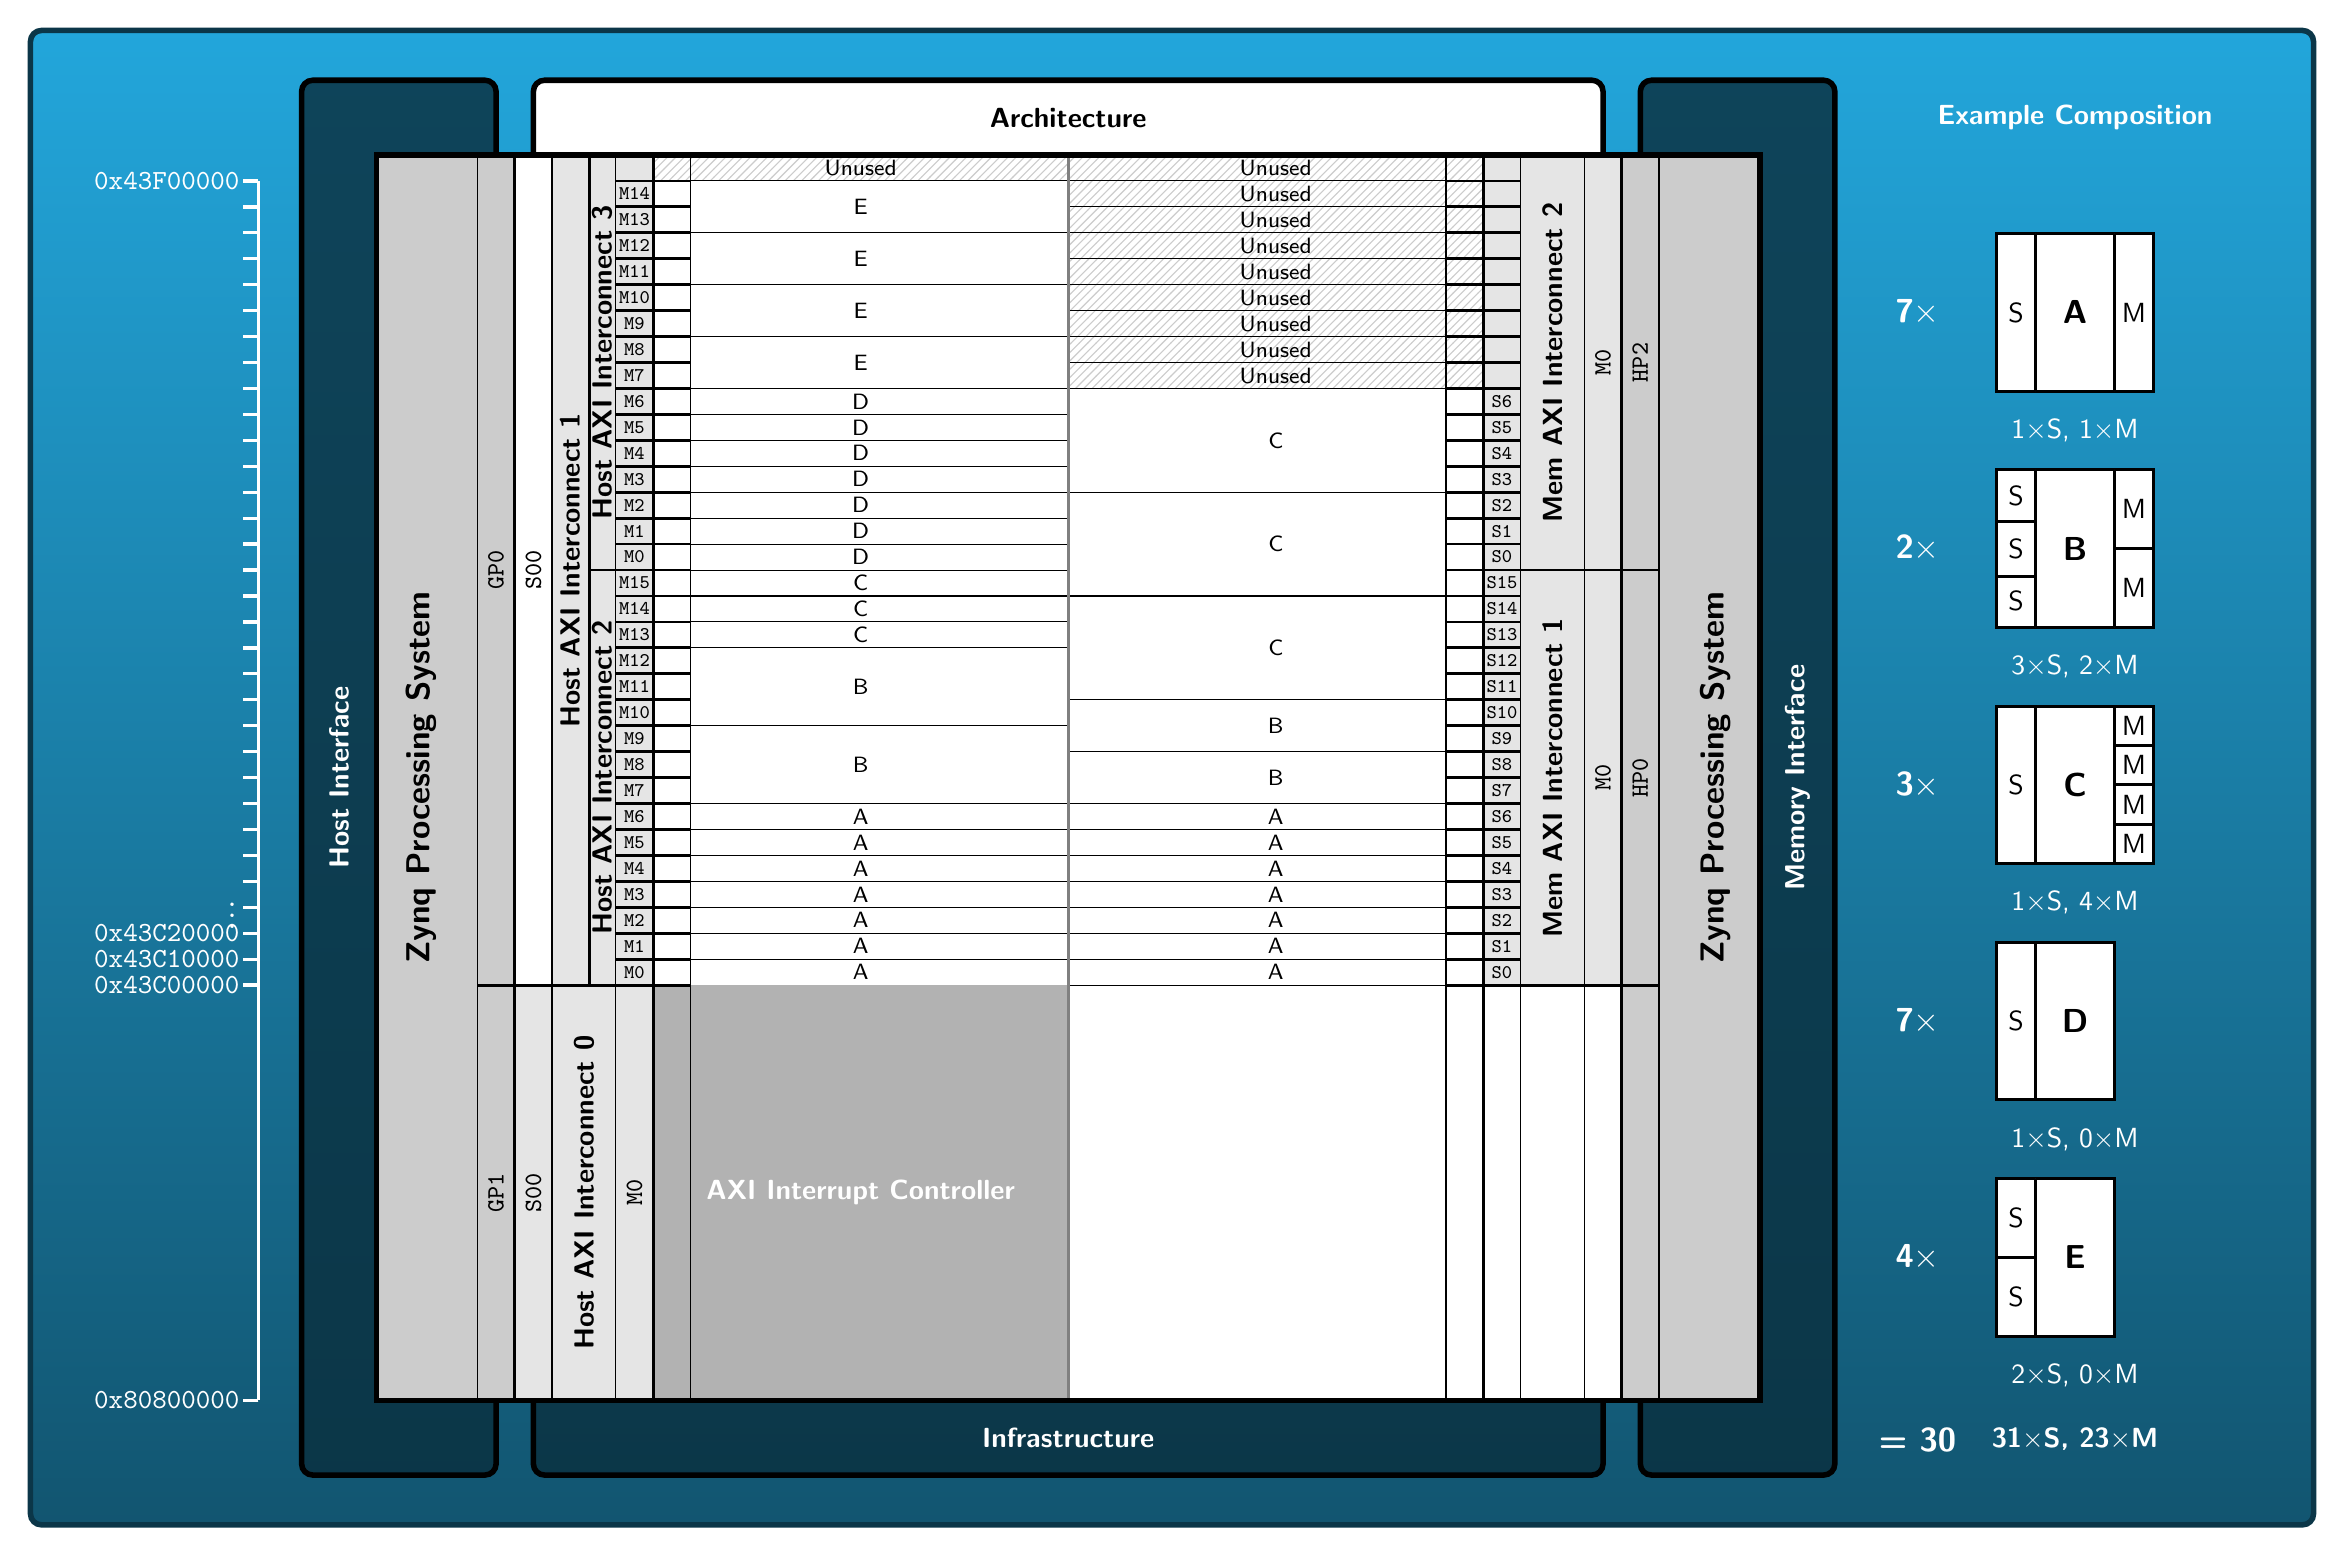
\begin{tikzpicture}[%
    outer border/.style={line width=2pt, draw=black},
    conn border/.style={line width=1pt, draw=black},
    ic border/.style={line width=1pt, draw=black},
    inner conn border/.style={line width=0.5pt, draw=black},
    inner ic border/.style={line width=0.5pt, draw=black},
    kernel label/.style={font=\footnotesize},
    kernel shape/.style={fill=white, draw=black},
    unused/.style={pattern=north east lines, pattern color=black!20},
    interconnect/.style={fill=black!10},
    interconnect label/.style={font=\bfseries, rotate=90},
    zynq/.style={fill=black!20},
    zynq label/.style={font=\large\bfseries, rotate=90},
    intc/.style={fill=black!30},
    intc label/.style={font=\bfseries\color{white}},
    zynq interface/.style={font=\small\ttfamily},
    part label/.style={font=\bfseries\color{white}},
    address/.style={font=\bfseries\ttfamily\color{white}, anchor=east},
    address bar/.style={very thick, white},
    platform box/.style={rounded corners, fill=esa5, bottom color=esa5, draw=black, line width=2pt,top color=esa4},
    arch box/.style={rounded corners, fill=white, draw=black, line width=2pt},
    frame box/.style={rounded corners, fill=esa3, top color=esa0, bottom color=esa3, draw=esa5, line width=2pt}
  ]%
  \def\totalheight{450pt}
  \def\totalwidth{500pt}
  \def\interfacefactor{0.03125} % 1/32
  \def\interfaceheight{($(t)!\interfacefactor!(hlb)$)}
  \def\zynqwidth{0.1*\totalwidth}
  \def\icwidth{\zynqwidth}
  \def\connwidth{0.27*\zynqwidth}
  \def\outerwidth{2*\connwidth}

  % axes on Y
  \coordinate (t) at (0,0);
  \coordinate (b) at (0, -\totalheight);
  \coordinate (m) at ($(t)!.5!(b)$);
  \coordinate (h0b) at ($(t)!.3333!(b)$);
  \coordinate (h1b) at ($(t)!.6666!(b)$);
  \foreach \n in {0, ..., 32}
    \coordinate (if\n) at ($(t)!\n*\interfacefactor!(h1b)$);
 
  % axes on X
  \coordinate (l) at (0,0);
  \coordinate (r) at (\totalwidth, 0);
  \coordinate (c) at ($(l)!.5!(r)$);
  \coordinate (zl) at ($(l) + (\zynqwidth,0)$);
  \coordinate (zr) at ($(r) - (\zynqwidth,0)$);
  \coordinate (icl) at ($(zl) + (\icwidth,0)$);
  \coordinate (icr) at ($(zr) - (\icwidth,0)$);

  \coordinate (zil) at ($(zl) - (\connwidth,0)$);
  \coordinate (zir) at ($(zr) + (\connwidth,0)$);

  \coordinate (icli) at ($(zl) + (\connwidth,0)$);
  \coordinate (icri) at ($(zr) - (\connwidth,0)$);

  \coordinate (iclm) at ($(icl) - (\connwidth,0)$);
  \coordinate (icrm) at ($(icr) + (\connwidth,0)$);

  \begin{pgfonlayer}{background}
    % draw outermost box
    \coordinate (obtl) at (-.25*\totalwidth, 0.1*\totalheight);
    \coordinate (obbr) at (1.4*\totalwidth, -1.1*\totalheight);
    \draw [frame box] (obtl) rectangle (obbr);
    % make structure boxes
    \draw [arch box] (zl |- t) +(0.25*\outerwidth,\outerwidth) rectangle
      ($(zr |- h1b) +(-0.25*\outerwidth,0)$);
    \draw [platform box] (l |- t) +(-\outerwidth,\outerwidth) 
      rectangle ($(zl |- b) +(-.25*\outerwidth,-\outerwidth)$);
    \draw [platform box] (zr |- t) +(0.25*\outerwidth,\outerwidth)
      rectangle ($(r |- b) +(\outerwidth,-\outerwidth)$);
    \draw [platform box] (zl |- h1b) +(0.25*\outerwidth,0) rectangle
      ($(zr |-b) + (-0.25*\outerwidth,-\outerwidth)$);

    % fill main background white
    \path [fill=white] (t -| l) rectangle (b -| r);

    % outer labels of four parts
    \node [part label, yshift=.5*\outerwidth, font=\bfseries] at (t -| c) {Architecture};
    \node [part label, rotate=90, yshift=0.5*\outerwidth] at (l |- m) {Host Interface};
    \node [part label, rotate=90, yshift=-0.5*\outerwidth] at (r |- m) {Memory Interface};
    \node [part label, yshift=-.5*\outerwidth] at (b -| c) {Infrastructure};
  \end{pgfonlayer}

  \begin{pgfonlayer}{background}
  % core slaves
  \begin{scope}[every node/.style={kernel label}, every path/.style={kernel shape}]
    \path [unused] (if0 -| icl) rectangle (if1 -| c) node [pos=0.5] {Unused};
    \foreach \x in {1, 3, ..., 8} {
      \mycount=\x
      \advance\mycount by 2
      \path (if\x -| icl) rectangle (if\the\mycount -| c) node [pos=0.5] {E};
    }
    \foreach \x in {9, 10, ..., 15} {
      \mycount=\x
      \advance\mycount by 1 
      \path (if\x -| icl) rectangle (if\the\mycount -| c) node [pos=0.5] {D};
    }
    \foreach \x in {16, 17, ..., 18} {
      \mycount=\x
      \advance\mycount by 1
      \path (if\x -| icl) rectangle (if\the\mycount -| c) node [pos=0.5] {C};
    }
    \foreach \x in {19, 22} {
      \mycount=\x
      \advance\mycount by 3
      \path (if\x -| icl) rectangle (if\the\mycount -| c) node [pos=0.5] {B};
    }
    \foreach \x in {25, 26, ..., 31} {
      \mycount=\x
      \advance\mycount by 1
      \path (if\x -| icl) rectangle (if\the\mycount -| c) node [pos=.5] {A};
    }
  \end{scope}
  
  % master interfaces
  \begin{scope}[every node/.style={kernel label}, every path/.style={kernel shape}]
    \foreach \x in {25, 26, ..., 31} {
      \mycount=\x
      \advance\mycount by 1
      \path (if\x -| c) rectangle (if\the\mycount -| icr) node [pos=.5] {A};
    }
    \foreach \x in {21, 23} {
      \mycount=\x
      \advance\mycount by 2 
      \path (if\x -| c) rectangle (if\the\mycount -| icr) node [pos=0.5] {B};
    }
    \foreach \x in {9, 13, ..., 17} {
      \mycount=\x
      \advance\mycount by 4 
      \path (if\x -| c) rectangle (if\the\mycount -| icr) node [pos=0.5] {C};
    }
    \foreach \x in {0, 1, ..., 8} {
      \mycount=\x
      \advance\mycount by 1
      \path [unused] (if\x -| c) rectangle (if\the\mycount -| icr) node [pos=0.5] {Unused};
    }
  \end{scope}

  % AXI interconnects
  \begin{scope}[every path/.style={interconnect}, every node/.style={interconnect label}]
    \path (zl |- t) ++(2*\connwidth,0) rectangle (icl |- h0b) node [pos=0.5, above] {Host AXI Interconnect 3};
    \path (zl |- h0b) ++(2*\connwidth,0) rectangle (icl |- h1b) node [pos=0.5, above] {Host AXI Interconnect 2};
    \path (zl |- t) ++(\connwidth,0) rectangle ($(icl |- h1b) +(-1.75*\connwidth,0)$) node [pos=0.5] {Host AXI Interconnect 1};
    \path (zl |- h1b) rectangle (icl |- b) node [pos=0.5] {Host AXI Interconnect 0};
    \path (icr |- t) rectangle (zr |- h0b) node [pos=0.5] {Mem AXI Interconnect 2};
    \path (icr |- h0b) rectangle (zr |- h1b) node [pos=0.5] {Mem AXI Interconnect 1};
  \end{scope}

  % Zynq PS7
  \begin{scope}[every path/.style={zynq}, every node/.style={zynq label}]
    \path (l |- t) rectangle (zl |- b) node [pos=0.5, anchor=south] {Zynq Processing System};
    \path (zr |- t) rectangle (r |- b) node [pos=0.5, anchor=north] {Zynq Processing System};
  \end{scope}

  % Zynq interfaces
  \begin{scope}[every node/.style={zynq interface, rotate=90}]
    \node at ($(zil |- t)!.5!(zl |- h1b)$) {GP0};
    %\node at ($(zil |- h0b)!.5!(zl |- h1b)$) {GP0};
    \node at ($(zil |- h1b)!.5!(zl |- b)$) {GP1};
    \node at ($(zr |- t)!.5!(zir |- h0b)$) {HP2};
    \node at ($(zr |- h0b)!.5!(zir |- h1b)$) {HP0};
  \end{scope}

  % AXI interfaces
  \begin{scope}[every node/.style={zynq interface, rotate=90}]
    \node at ($(zl |- t)!.5!(icli |- h1b)$) {S00};
    %\node at ($(zl |- h0b)!.5!(icli |- h1b)$) {S00};
    \node at ($(zl |- h1b)!.5!(icli |- b)$) {S00};
    \node at ($(iclm |- h1b)!.5!(icl |- b)$) {M0};
    \node at ($(zr |- t)!.5!(icri |- h0b)$) {M0};
    \node at ($(zr |- h0b)!.5!(icri |- h1b)$) {M0};
  \end{scope}

  % AXI host ic masters
  \begin{scope}[every node/.style={zynq interface, font=\scriptsize\ttfamily}]
    \foreach \n in {1, ..., 15} {
      \mycount=\n
      \advance\mycount by 1
      \numcount=15
      \advance\numcount by -\n
      \node at ($(iclm |- if\the\mycount)!.5!(icl |- if\n)$) {M\the\numcount};
      \ifnum \the\numcount < 7
      \node at ($(icr |- if\the\mycount)!.5!(icrm |- if\n)$) {S\the\numcount};
      \fi
    }
    \foreach \n in {16, ..., 31} {
      \mycount=\n
      \advance\mycount by 1
      \numcount=31
      \advance\numcount by -\n
      \node at ($(iclm |- if\the\mycount)!.5!(icl |- if\n)$) {M\the\numcount};
      \node at ($(icr |- if\the\mycount)!.5!(icrm |- if\n)$) {S\the\numcount};
    }
  \end{scope}

  % AXI Interrupt Controller
  \path [intc] (icl |- h1b) rectangle (c |- b) node [pos=0.5, intc label] {AXI Interrupt Controller};
  \end{pgfonlayer}

  \begin{pgfonlayer}{background}
    \path [outer border, line width=1pt, draw=black!50] (t -| c) -- (b -| c);
    \path [outer border] (t -| l) rectangle (b -| r);
    %\foreach \hb in {h0b, h1b}
      \path [ic border] (t -| zl) ++(2*\connwidth,0) -- ($(h1b -| zl) +(2*\connwidth,0)$);
      \path [ic border] 
        (h0b -| zil) ++(3*\connwidth,0) -- ($(h0b -| icl) + (\connwidth,0)$)
        (h0b -| icr) +(-\connwidth,0) -- (h0b -| zir);
      \path [ic border] 
        (h1b -| zil) -- ($(h1b -| icl) + (\connwidth,0)$)
        (h1b -| icr) +(-\connwidth,0) -- (h1b -| zir);
    \foreach \n in {1, ..., 31} {
      \path [ic border] (if\n -| iclm) -- ($(if\n -| icl) + (\connwidth,0)$);
      \path [ic border] (if\n -| icr) +(-\connwidth,0) -- (if\n -| icrm);
    }

    \foreach \connaxe in {zl, zr, icl, icr} {
      \path [conn border] (t -| \connaxe) -- (b -| \connaxe);
      \path [inner conn border]
        (t -| \connaxe) +(\connwidth, 0) -- ($(b -| \connaxe) +(\connwidth, 0)$)
        (t -| \connaxe) +(-\connwidth, 0) -- ($(b -| \connaxe) +(-\connwidth, 0)$);
    }

    % draw AXI address space bar
    \begin{scope}[every path/.style={address bar}, every node/.style={address}]
      \draw [very thick] (l |- if1) +(-1.5cm,0) -- ($(l |- b) + (-1.5cm,0)$);
      \foreach \x in {t, m, b} \draw (\x |- b) ++(-1.5cm, 0) -- +(-2mm,0);
      \foreach \x in {1, ..., 32} \draw (if\x -| l) ++(-1.5cm, 0) -- +(-2mm,0);
      \node at ($(l |- b) +(-1.6cm, 0)$) {0x80800000};
      \foreach \x/\addr in {32/0x43C00000, 31/0x43C10000, 30/0x43C20000, 29/\vdots, 1/0x43F00000}
        \node at ($(l |- if\x) +(-1.6cm, 0)$) {\addr};
    \end{scope}

    \coordinate (compo) at ($(r |- t) +(3cm,-1cm)$);
    \coordinate (compol) at ($(compo) +(-1cm,0)$);

    \begin{scope}[line width=1.1pt, every node/.style={font=\large\bfseries}]
      \node [part label, font=\bfseries\color{white}, yshift=0.5*\outerwidth] at ($(compo |- t) +(1cm,0)$) {Example Composition};
      \foreach \x/\l/\n/\s/\m in {0/A/7/1/1, 1/B/2/3/2, 2/C/3/1/4, 3/D/7/1/0, 4/E/4/2/0} {
        \ifnum \m > 0
        \draw [fill=white] (compo) ++(0,\x*-3cm) rectangle +(2cm,-2cm) node [pos=.5] {\l};
	\else
        \draw [fill=white] (compo) ++(0,\x*-3cm) rectangle +(1.5cm,-2cm) node [pos=.5, xshift=.25cm] {\l};
	\fi
	\draw [fill=white] (compo) ++(0.5cm,\x*-3cm) -- +(0,-2cm);
	\ifnum \m > 0
	\draw [fill=white] (compo) ++(1.5cm,\x*-3cm) -- +(0,-2cm);
	\fi
	\node [font=\large\bfseries\color{white}] at ($(compol) + (0,\x*-3cm -1cm)$) {\n $\times$};
        \node [font=\color{white}] at ($(compo) +(1cm,\x*-3cm -2.5cm)$) {\s$\times$S, \m$\times$M};
      }
      % A
      \node [font=] at ($(compo) +(0.25cm,-1cm)$) {S};
      \node [font=] at ($(compo) +(1.75cm,-1cm)$) {M};
      % B
      \draw (compo) ++(0,-3.65cm) -- +(0.5cm,0);
      \draw (compo) ++(0,-4.35cm) -- +(0.5cm,0);
      \draw (compo) ++(1.5cm,-4cm) -- +(0.5cm,0);
      \node [font=] at ($(compo) +(0.25cm,-3.33cm)$) {S};
      \node [font=] at ($(compo) +(0.25cm,-4cm)$) {S};
      \node [font=] at ($(compo) +(0.25cm,-4.66cm)$) {S};
      \node [font=] at ($(compo) +(1.75cm,-3.5cm)$) {M};
      \node [font=] at ($(compo) +(1.75cm,-4.5cm)$) {M};
      % C
      \draw (compo) ++(1.5cm,-6.5cm) -- +(0.5cm,0);
      \draw (compo) ++(1.5cm,-7cm) -- +(0.5cm,0);
      \draw (compo) ++(1.5cm,-7.5cm) -- +(0.5cm,0);
      \node [font=] at ($(compo) +(0.25cm,-7cm)$) {S};
      \node [font=] at ($(compo) +(1.75cm,-6.25cm)$) {M};
      \node [font=] at ($(compo) +(1.75cm,-6.75cm)$) {M};
      \node [font=] at ($(compo) +(1.75cm,-7.25cm)$) {M};
      \node [font=] at ($(compo) +(1.75cm,-7.75cm)$) {M};
      % D
      %\fill [pattern=north east lines] (compo) ++(1.5cm,-9cm) rectangle +(0.5cm,-2cm);
      \node [font=] at ($(compo) +(0.25cm,-10cm)$) {S};
      % E
      \draw (compo) ++(0,-13cm) -- +(0.5cm,0);
      \node [font=] at ($(compo) +(0.25cm,-12.5cm)$) {S};
      \node [font=] at ($(compo) +(0.25cm,-13.5cm)$) {S};
      %\fill [pattern=north east lines] (compo) ++(1.5cm,-12cm) rectangle +(0.5cm,-2cm);
      % sum
      \node [font=\large\bfseries\color{white}] at ($(compol |- b) +(0,-.5cm)$) {= 30};
      \node [font=\bfseries\color{white}] at ($(compo |- b) +(1cm,-.5cm)$) {31$\times$S, 23$\times$M};
    \end{scope}

  \end{pgfonlayer}
\end{tikzpicture}
\end{document}
